\documentclass{beamer}[10pt, usepdftitle=false, handout]

\beamertemplatenavigationsymbolsempty

\usepackage[T1]{fontenc}
\usepackage[]{algorithm2e}
\usepackage{multimedia}
\usepackage{gensymb}
\usepackage{textcomp}

%\usepackage[font=small,labelfont=bf]{caption} 

\usetheme{Boadilla}

\title{Basic of Computer Networks 4}
\author[]{Paul Blondel}
\institute[]{CNAM}
\date[]{March 1st, 2019}

\usepackage[style=british]{csquotes}


\def\signed #1{{\leavevmode\unskip\nobreak\hfil\penalty50\hskip1em
  \hbox{}\nobreak\hfill #1%
  \parfillskip=0pt \finalhyphendemerits=0 \endgraf}}

\newsavebox\mybox
\newenvironment{aquote}[1]
  {\savebox\mybox{#1}\begin{quote}\openautoquote\hspace*{-.7ex}}
  {\unskip\closeautoquote\vspace*{1mm}\signed{\usebox\mybox}\end{quote}}


\setbeamertemplate{headline}
{
  \leavevmode%
  \hbox{%
  \begin{beamercolorbox}[wd=1.0\paperwidth,ht=2.25ex,dp=1ex,center]{author in head/foot}%
    \usebeamerfont{author in head/foot}\insertsubsection
  \end{beamercolorbox}}%
  \vskip0pt%
}


\setbeamertemplate{footline}
{
  \leavevmode%
  \hbox{%
  \begin{beamercolorbox}[wd=.5\paperwidth,ht=2.25ex,dp=1ex,center]{author in head/foot}%
    \usebeamerfont{author in head/foot}\insertsection
  \end{beamercolorbox}%
  \begin{beamercolorbox}[wd=.5\paperwidth,ht=2.25ex,dp=1ex,center]{title in head/foot}%
    \usebeamerfont{title in head/foot} \inserttitle \hspace*{2em}  \insertframenumber{} / \inserttotalframenumber\hspace*{2ex} 
  \end{beamercolorbox}}%
  \vskip0pt%
}

\AtBeginSection[]
{
   \begin{frame}
    \tableofcontents[ 
    currentsection] 
   \end{frame}
}

\begin{document}
	{
	\setbeamertemplate{footline}{
  	\leavevmode%
  	\hbox{%
  	\begin{beamercolorbox}[wd=.5\paperwidth,ht=2.25ex,dp=1ex,center]{author in head/foot}%
  	\end{beamercolorbox}%
  	\begin{beamercolorbox}[wd=.5\paperwidth,ht=2.25ex,dp=1ex,center]{title in head/foot}%
  	\end{beamercolorbox}}%
  	\vskip0pt%	
	} 
	\begin{frame}
	\titlepage
	\end{frame}

	\begin{frame}
	
	\begin{aquote}{Tim-Bernes Lee - Creator of the WEB}
I think, in general, it's clear that most bad things come from misunderstanding, and communication is generally the way to resolve misunderstandings — and the Web's a form of communications — so it generally should be good.
	\end{aquote}	
	
	\end{frame}


	\begin{frame}
		\tableofcontents
	\end{frame}
	}

	\addtocounter{framenumber}{-3}

	\section{Network model}
	%\subsection{What is it?}

    \begin{frame}[label=(first)]
	
	What is a network model?
	\vspace*{1em}
	
	\begin{itemize}
	\item{It is a method for describing and analyzing data communication networks by breaking the entire set of communication process into a number of layers}
	\item{Each layer has a specific function (there will be described later)}
	\end{itemize}
	
	
	\end{frame}
	
	\section{The OSI model}

	\subsection{The OSI model}
	
	\begin{frame}
	
	The OSI model was an attempt to unify every network models. Nowadays it is especially a theoretical model people use as a reference model. 
	\vspace*{1em}
	
	\begin{itemize}
	\item{International standard organization (ISO) established a commitee in 1977 to develop an architecture for systems communication}
	\item{The Open System Interconnection (OSI) reference model is the result of this effort.}
	\item{This model allows any two different systems to communicate regardless of their underlying architecture.}
	
	\end{itemize}
	
	\end{frame}
	
	\subsection{OSI model: what for?}
	
	\begin{frame}
	
	The OSI model ...	
	\vspace*{1em}	
	
	\begin{itemize}
	\item{... describes how data flows from one computer, through a network to another computer.}	
	\item{... is not a protocol; it is a model for understanding and designing a network architecture that is flexible and robust.}
	\item{... consists of seven separate but related layers, each of which defines a part of the process of moving information across a network.}
	\end{itemize}		
	
	\end{frame}
	
	 \subsection{The OSI model: show me the layers!}
	 
	 \begin{frame}
	 
	The OSI model is made of seven layers:
	\vspace*{1em}
	
	\begin{center}	
	\begin{figure}
		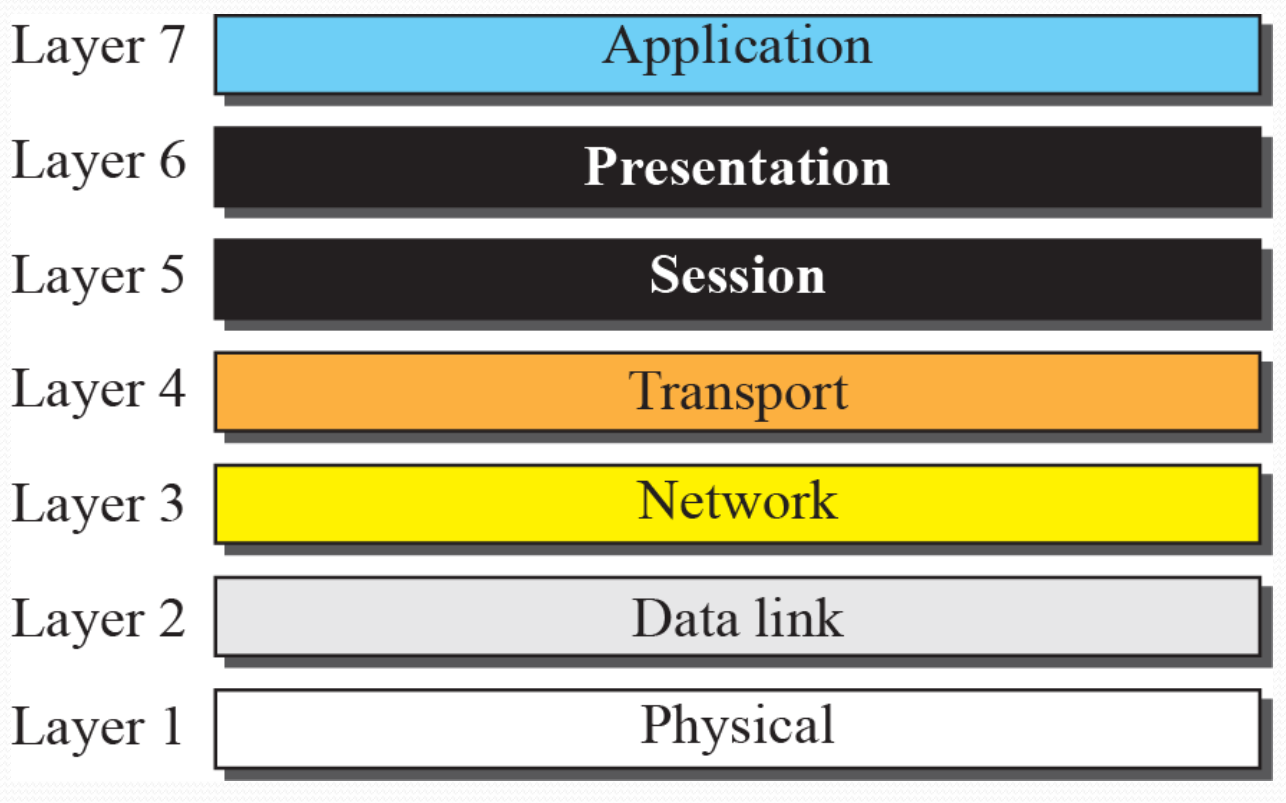
\includegraphics[scale=0.3]{images/4-1.png} 
     	%\vspace*{-0.5em}
		%\caption{Floating gate transistor cell}
	\end{figure}	
	\end{center}	 
	 
		  
	 \end{frame}	  
	 
	\begin{frame}
	
	Looks like that, right?
	\vspace*{1em}	
	
	\begin{center}	
	\begin{figure}
		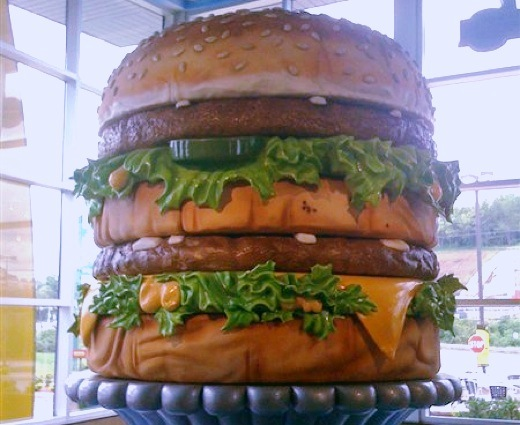
\includegraphics[scale=0.5]{images/4-3.png} 
     	%\vspace*{-0.5em}
		%\caption{Floating gate transistor cell}
	\end{figure}	
	\end{center}
	
	
	\end{frame}	 
	 
	 
	 \begin{frame}
	 
	Why so many layers?
	\vspace*{1em}	
	
	\begin{itemize}
	\item{To reduce the complexity, networks are organized as a stack of layers, one below the other.}
	\item{Each layer is responsible for a specific task, it provides a services to an adjacent layer.}
	\end{itemize}		 
	 
	
	 \end{frame}

	\begin{frame}
	
	\begin{center}	
	\begin{figure}
		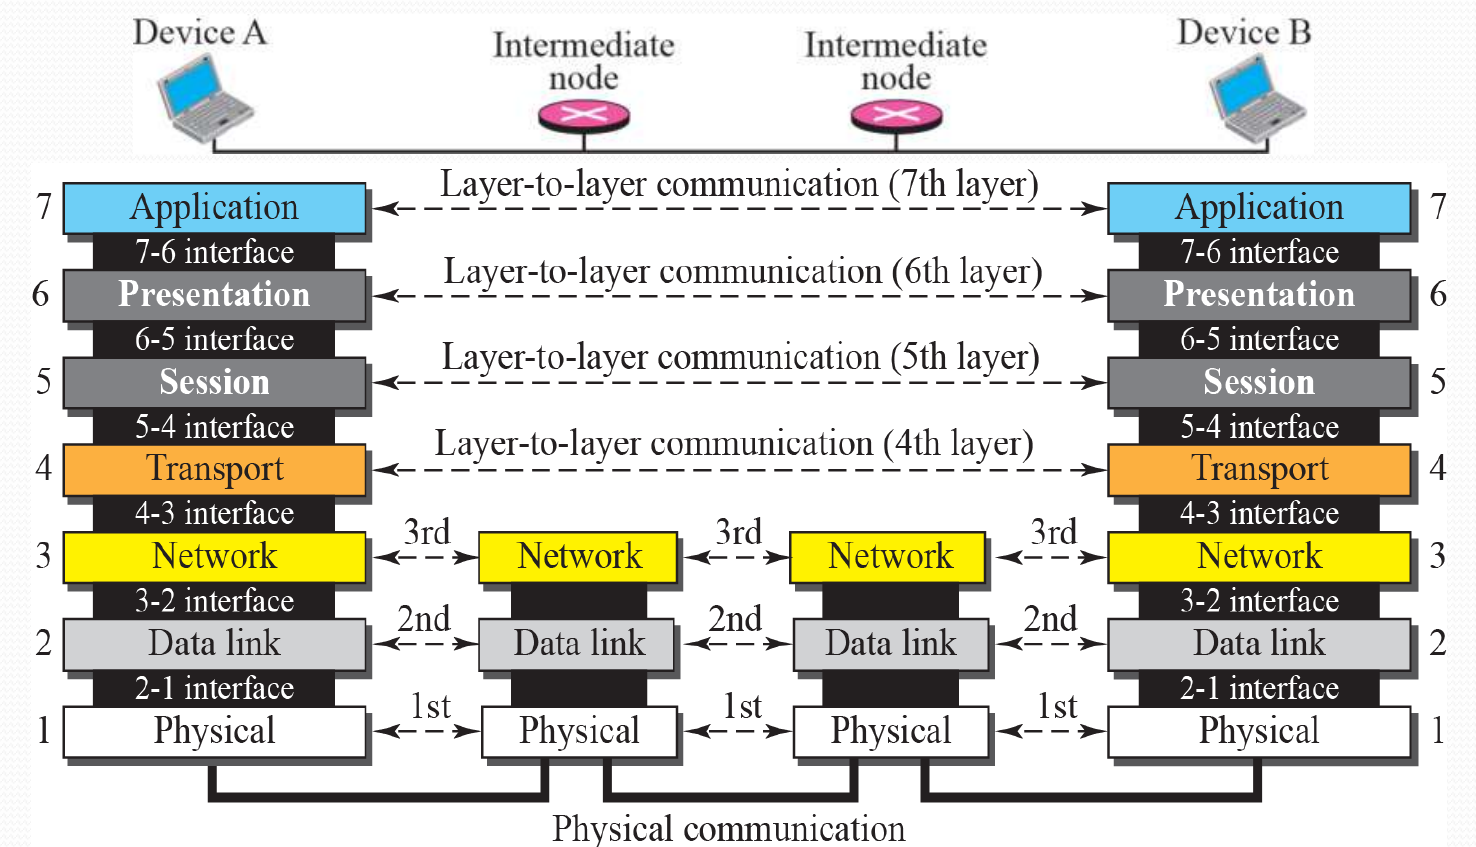
\includegraphics[scale=0.3]{images/4-2.png} 
     	%\vspace*{-0.5em}
		%\caption{Floating gate transistor cell}
	\end{figure}	
	\end{center}
	
	\end{frame}
		
	\begin{frame}
	
	Three subgroups of layers:	
	\vspace*{1em}	
	
	\begin{itemize}
	\item{Lower layers: physical, data link and network layers are network support layers (responsible for data transmission).}	
	\item{Middle layer: the transport layer links the two subgroups of layers.}
	\item{Higher layers: session, presentation and application layers are user support layers (responsible for application working).}	
	\end{itemize}		
	
	\end{frame}

	\begin{frame}
	
	Example of exchange using the OSI model:
	\vspace*{1em}	
	
		\begin{center}	
	\begin{figure}
		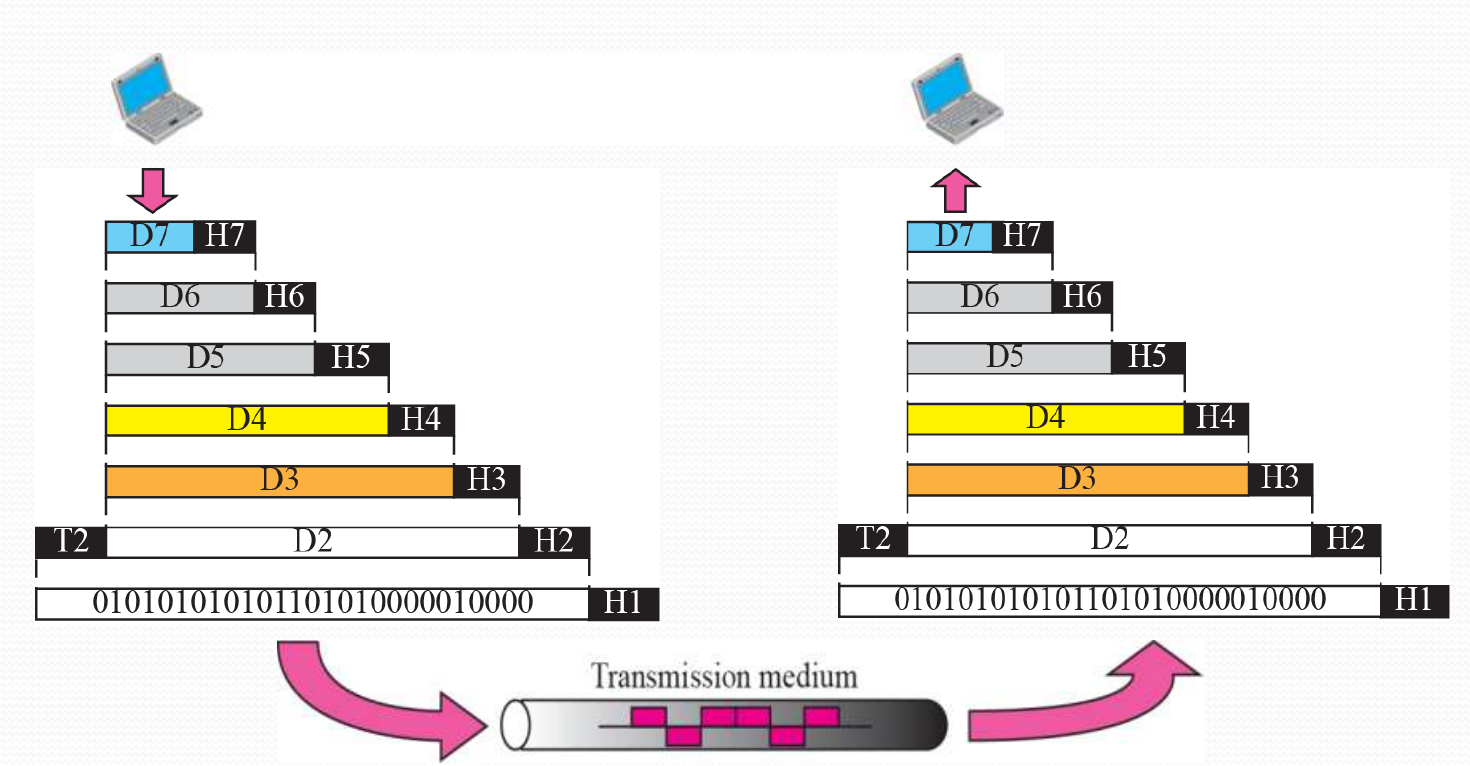
\includegraphics[scale=0.3]{images/4-4.png} 
     	%\vspace*{-0.5em}
		%\caption{Floating gate transistor cell}
	\end{figure}	
	\end{center}
	
	\end{frame}

	\subsection{More details about the layers}

	\begin{frame}
	
	Layer 1: the physical layer
	\vspace*{1em}	
	
	\begin{itemize}
	\item{First layer of the OSI model: all the information of all the other layers go through this layer.}	
	\item{It is responsible for the actual physical connection between the devices! (ex: cable, WI-FI, etc.)}
	\item{Thanks to this layer: individual bits can go from one node (=computer) to the next!}
	\end{itemize}		
	\vspace*{0.5em}	
	
	\begin{block}{Note}
	System administrators use to say that most network connection problems occur because of this layer! Typically someone unplugged the cable by mistake!	
	\end{block}
		
	\end{frame}
	
	\begin{frame}
	
	The physical layer "contains" the data link layer like this:
	\vspace*{1em}	
	
	\begin{center}	
	\begin{figure}
		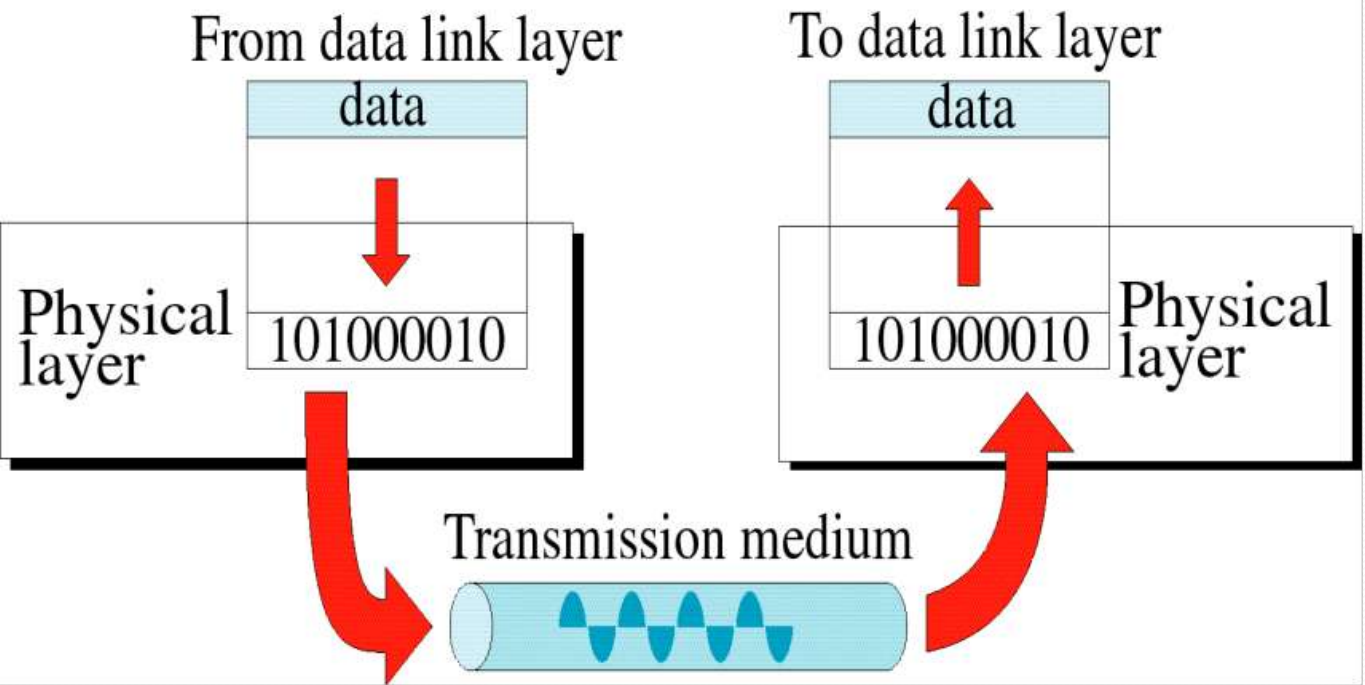
\includegraphics[scale=0.3]{images/4-5.png} 
     	%\vspace*{-0.5em}
		%\caption{Floating gate transistor cell}
	\end{figure}	
	\end{center}
	
	
	\end{frame}
	
	\begin{frame}
	
	The functions of the physical layer are very low-levels:
	\vspace*{1em}	
	
	\begin{itemize}
	\item{Converting bits to signals}
	\item{Bit synchronization}
	\item{Manage physical connection}
	\item{Bit rate control}
	\item{Line configuration}
	\item{Physical topology}
	\item{Transmission mode}
	\item{Multiplexing}
	\item{Switching}	
	\end{itemize}		
		
	\end{frame}
	
	\begin{frame}
	
	Layer 2: the data link layer
	\vspace*{1em}	
	
	The data link layer is responsible for moving frames (=blocks of data) from one node to the next.
	\vspace*{0.5em}	
	
	\begin{center}	
	\begin{figure}
		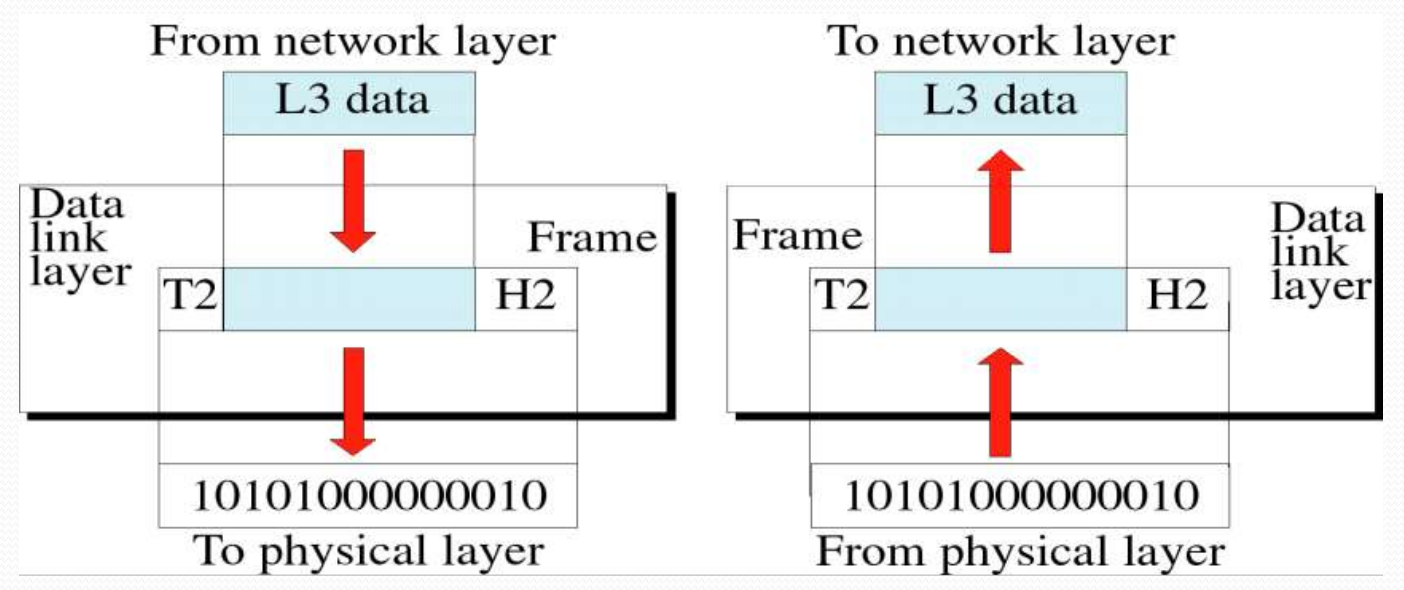
\includegraphics[scale=0.3]{images/4-6.png} 
     	%\vspace*{-0.5em}
		%\caption{Floating gate transistor cell}
	\end{figure}	
	\end{center}
				
	\end{frame}	

	\begin{frame}
	
	The functions of the data link layer are:
	\vspace*{1em}	
	
	\begin{itemize}
	\item{Framing: dividing the data from the network layer info frames (blocks)}
	\item{Physical addressing: add a header to the frame to define the physical address (MAC) of the source and the destination machines}
	\item{Flow control: it is the traffic regulatory mechanism implemented by this layer that prevents the faster sender from drowning a slower receiver}
	\item{Error control: it provides the mechanism of error control in which it detects and re-transmits damaged of lost frames.}
	\item{Feedback: transmitting the frames, the system waits for the feedback.}
	\end{itemize}		
	
	\end{frame}

	\begin{frame}
	
	The layer 3: the network layer
	\vspace*{1em}	
	
	\begin{center}	
	\begin{figure}
		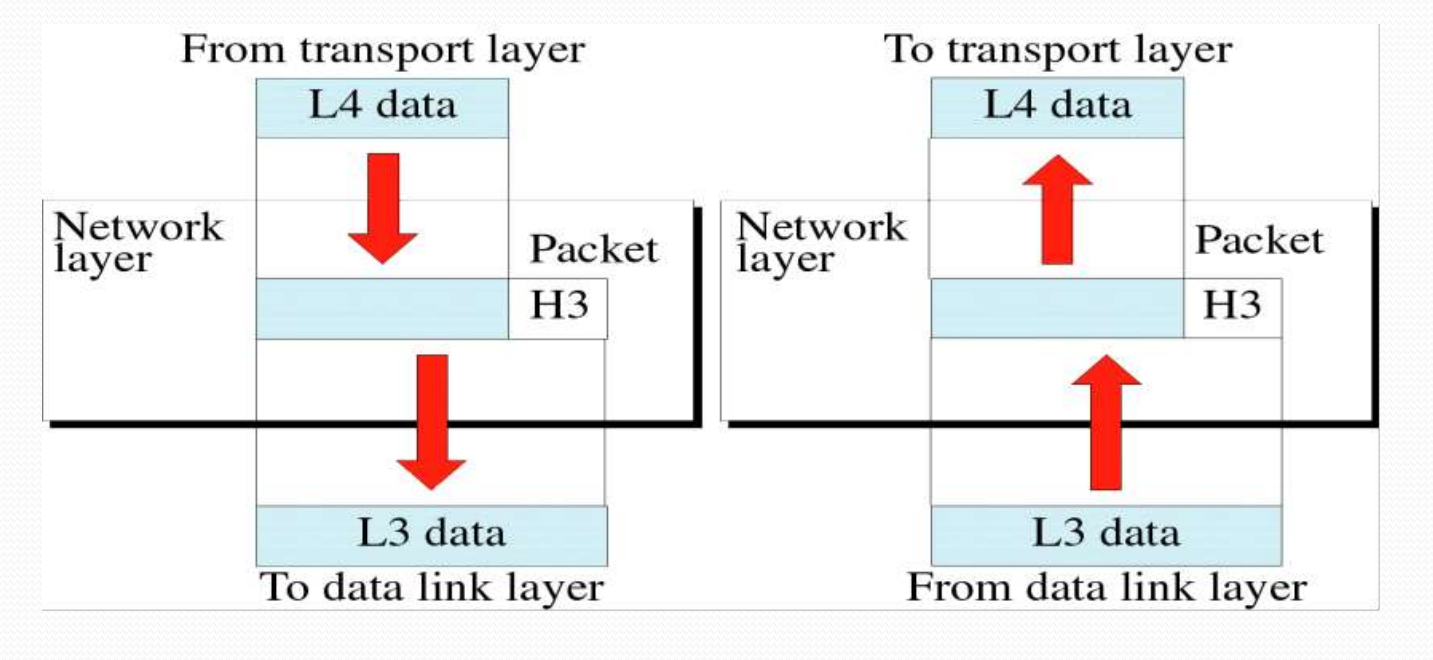
\includegraphics[scale=0.3]{images/4-7.png} 
     	%\vspace*{-0.5em}
		%\caption{Floating gate transistor cell}
	\end{figure}	
	\end{center}
	
	
	\end{frame}

	\begin{frame}
	
	The functions of the network layer:
	\vspace*{1em}	
	
	\begin{itemize}
	\item{It is responsible for the source to destination delivery of a packet across multiple networks.}
	\item{Routing: provide mechanism to transmit data over independent networks that are linked together (typically passing from router to router. Ex: from a local network to another local network passing through WLAN).}
	\item{Logical addressing: adds logical addresses of sender and receiver (require a new addressing system to permit transmission of data through independent networks).}	
	\end{itemize}		
	
	\end{frame}

	\begin{frame}
	
	The layer 4: the transport layer	
	\vspace*{1em}	
	
	The transport layer is responsible for source process to destination process delivery of entire message.
	\vspace*{0.5em}			
			
		\begin{center}	
	\begin{figure}
		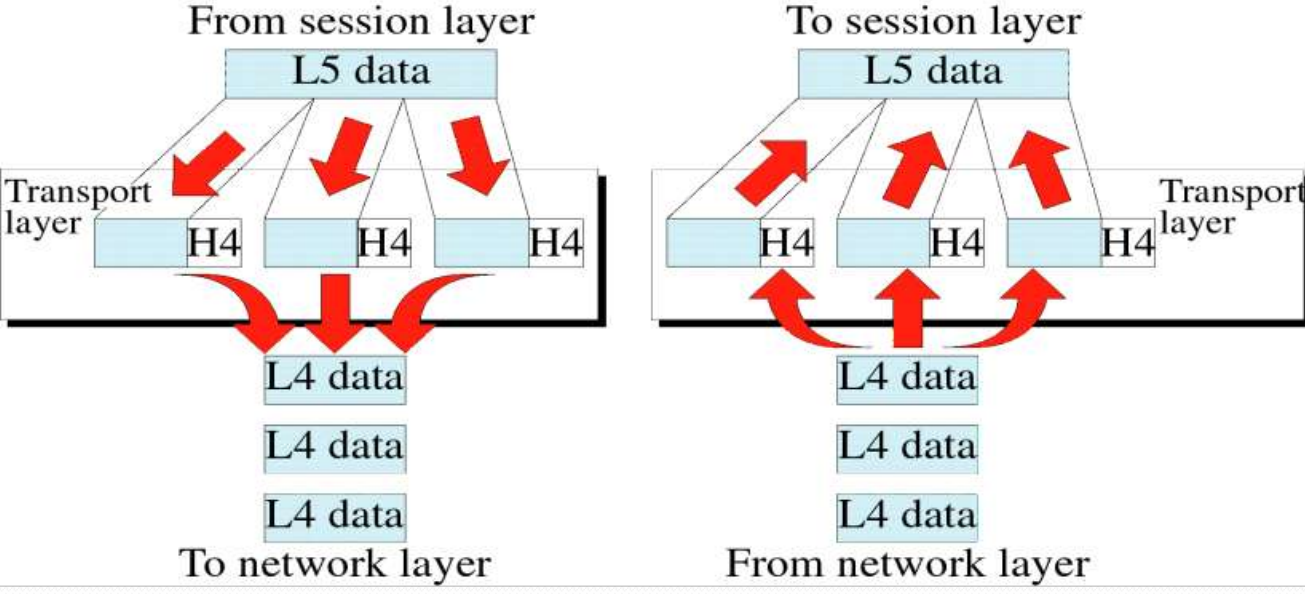
\includegraphics[scale=0.3]{images/4-8.png} 
     	%\vspace*{-0.5em}
		%\caption{Floating gate transistor cell}
	\end{figure}	
	\end{center}
	
	
	\end{frame}

	\begin{frame}
	
	The transport layer provides two types of services:
	\vspace*{1em}	
	
	\begin{enumerate}
	\item{Connection Oriented Transmission: In this type of transmission the receiving device sends an acknowledgment back to the source after a packet or group of packet is received.}
	\item{Connection-less Transmission: In this type of transmission the receiver does not acknowledge receipt of a packet.}
	\end{enumerate}
		
	\end{frame}

	\begin{frame}
	
	The functions of the transport layer:
	\vspace*{1em}	
	
	\begin{itemize}
	\item{Segmentation and Reassembly: Divide the message received from Session layer into Segments and number them to make a sequence for reassembly at the receiving side.}
	\item{Serviced point addressing: This layer makes sure that the messages is delivered to the correct process on destination machine.}
	\item{Error control: Make sure that the entire message arrives without errors else re-transmit.}	
	\item{Flow control: Transport layer makes sure that the sender and the receiver communicate at a rate they both can handle.}	
	
	\end{itemize}		
	
	\end{frame}
	
	\begin{frame}
	
	The layer 5: the session layer
	\vspace*{1em}	
	
	It is responsible for beginning, maintaining and ending the communication between two devices, which is called session.
	\vspace*{0.5em}	
	
		\begin{center}	
	\begin{figure}
		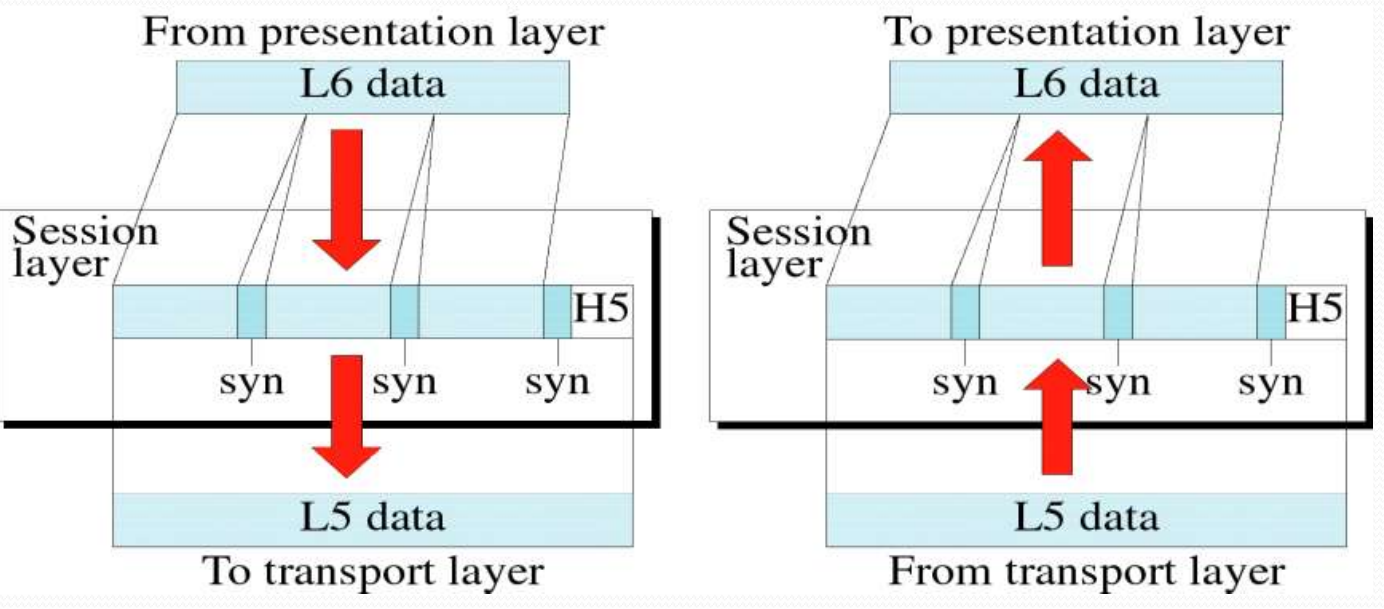
\includegraphics[scale=0.3]{images/4-9.png} 
     	%\vspace*{-0.5em}
		%\caption{Floating gate transistor cell}
	\end{figure}	
	\end{center}
	
	
	\end{frame}	
	
	\begin{frame}
	
	Functions of the session layer:
	\vspace*{1em}	
	
	\begin{itemize}
	\item{Establishment, maintaining and ending a session:
		\begin{itemize}
			\item{Sends SYN packet - establish request}
			\item{Receives ACK \& SYN - established}
			\item{To end - sender sends ACK}
		\end{itemize}		
	}
	\item{Dialog Control: The session layer allows systems to enter into a dialog}
	\item{Synchronization: Allows a process to add checkpoints to a stream of data.}	
	\end{itemize}		
		
	
	
	\end{frame}
	
	\begin{frame}
	
	The layer 6: the presentation layer
	\vspace*{1em}	
	
	This layer is concerned with the syntax and semantics of the information exchanged between two systems.	
	\vspace*{0.5em}	
	
			\begin{center}	
	\begin{figure}
		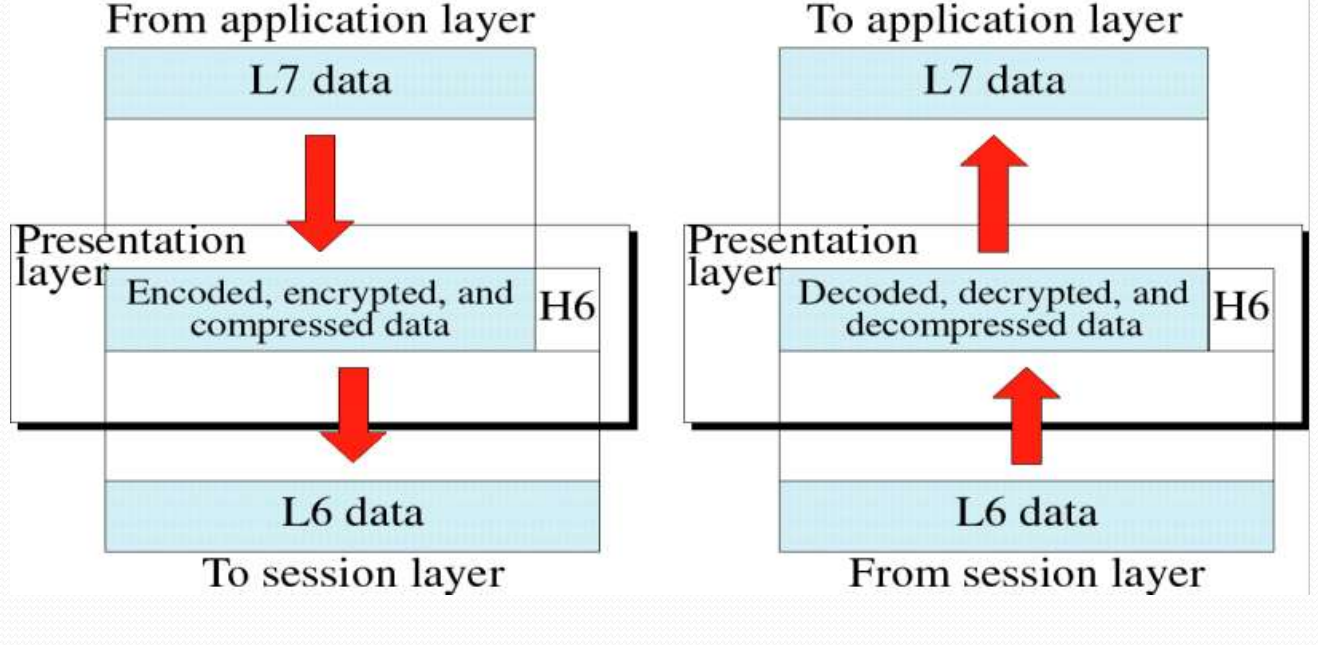
\includegraphics[scale=0.3]{images/4-10.png} 
     	%\vspace*{-0.5em}
		%\caption{Floating gate transistor cell}
	\end{figure}	
	\end{center}
		
	
	
	\end{frame}	
	
	\begin{frame}
	
	Functions of presentation layer:
	\vspace*{1em}	
	
	\begin{itemize}
		
	\item{Data Translation: Encoding and Decoding Sender to Common format on Sending side Common to Receiving format on Receiver side}
	
	\item{Data Encryption: For security and privacy purpose}
	
	\item{Data Compression: Data compression reduces the number of bits contained in the information}
	
	\end{itemize}		
	
	In practice, few existing network models have a presentation layer ...		
		
	
	\end{frame}
	
	\begin{frame}
	
	The layer 7: the application layer	
	\vspace*{1em}	
	
	It provides user interfaces and/or support for services, like e-mail, file transfer.
	\vspace*{0.5em}	
	
				\begin{center}	
	\begin{figure}
		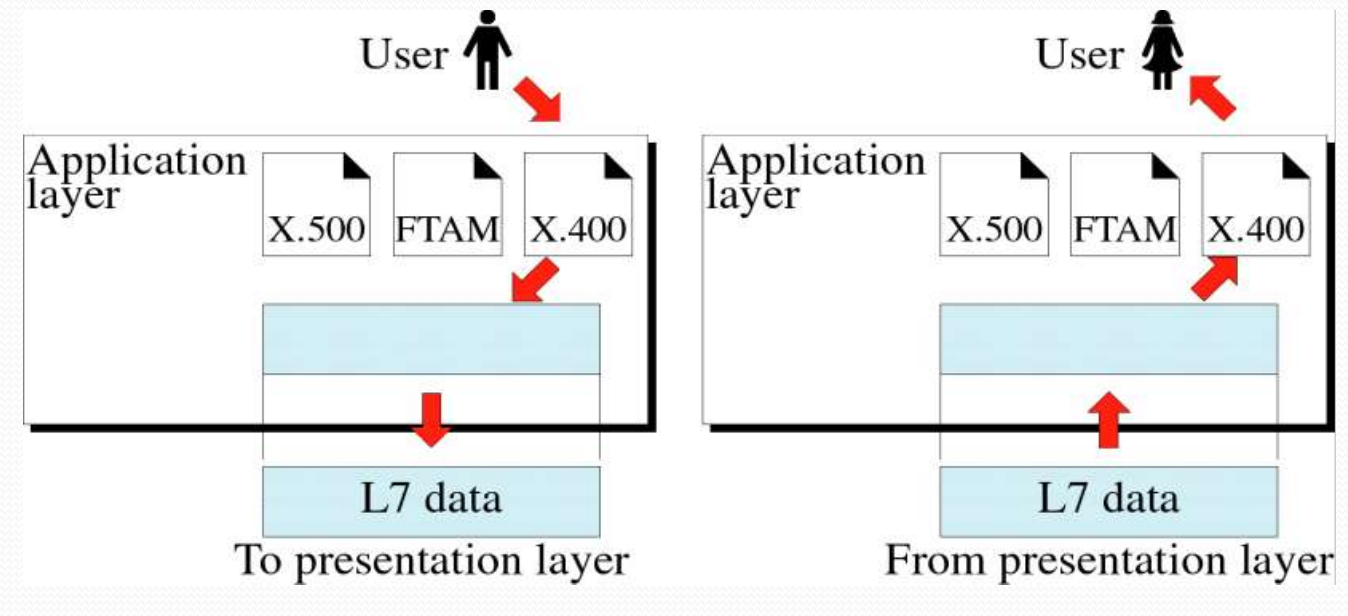
\includegraphics[scale=0.3]{images/4-11.png} 
     	%\vspace*{-0.5em}
		%\caption{Floating gate transistor cell}
	\end{figure}	
	\end{center}
	
	
	\end{frame}
	
	\begin{frame}
	
	Functions of the application layer:
	\vspace*{1em}	
	
	\begin{itemize}
	\item{Network Virtual terminal: It allows a user to log on to a remote host}
	\item{File Transfer Access, and Management: This application allows a user to access files in a remote host.}
	\item{Mail Services: This application provides various e-mail services.} 
	\item{Directory Services: This application provides the distributed database sources and access for global information about various objects and services.}
	\end{itemize}
	
	\end{frame}
	
	\section{The TCP/IP Model}
	\subsection{What is it?}	
	
	\begin{frame}
	
	The TCP/IP model ...
	\vspace*{1em}	
	
	\begin{itemize}
	\item{... forms the base of present day internet!}
	\item{... is made of two protocols: TCP and IP}
	\item{... is was initially used by ARPANET}
	\item{... is made of four layers:
		\begin{enumerate}
			\item{Host-to-network}
			\item{Internet}
			\item{Transport}
			\item{Application}
		\end{enumerate}			
	}	
	\end{itemize}
	
	\end{frame}

	\subsection{TCP/IP and OSI Model compared}

	\begin{frame}
	
	TCP/IP and OSI Model compared:
	\vspace*{1em}	
	
					\begin{center}	
	\begin{figure}
		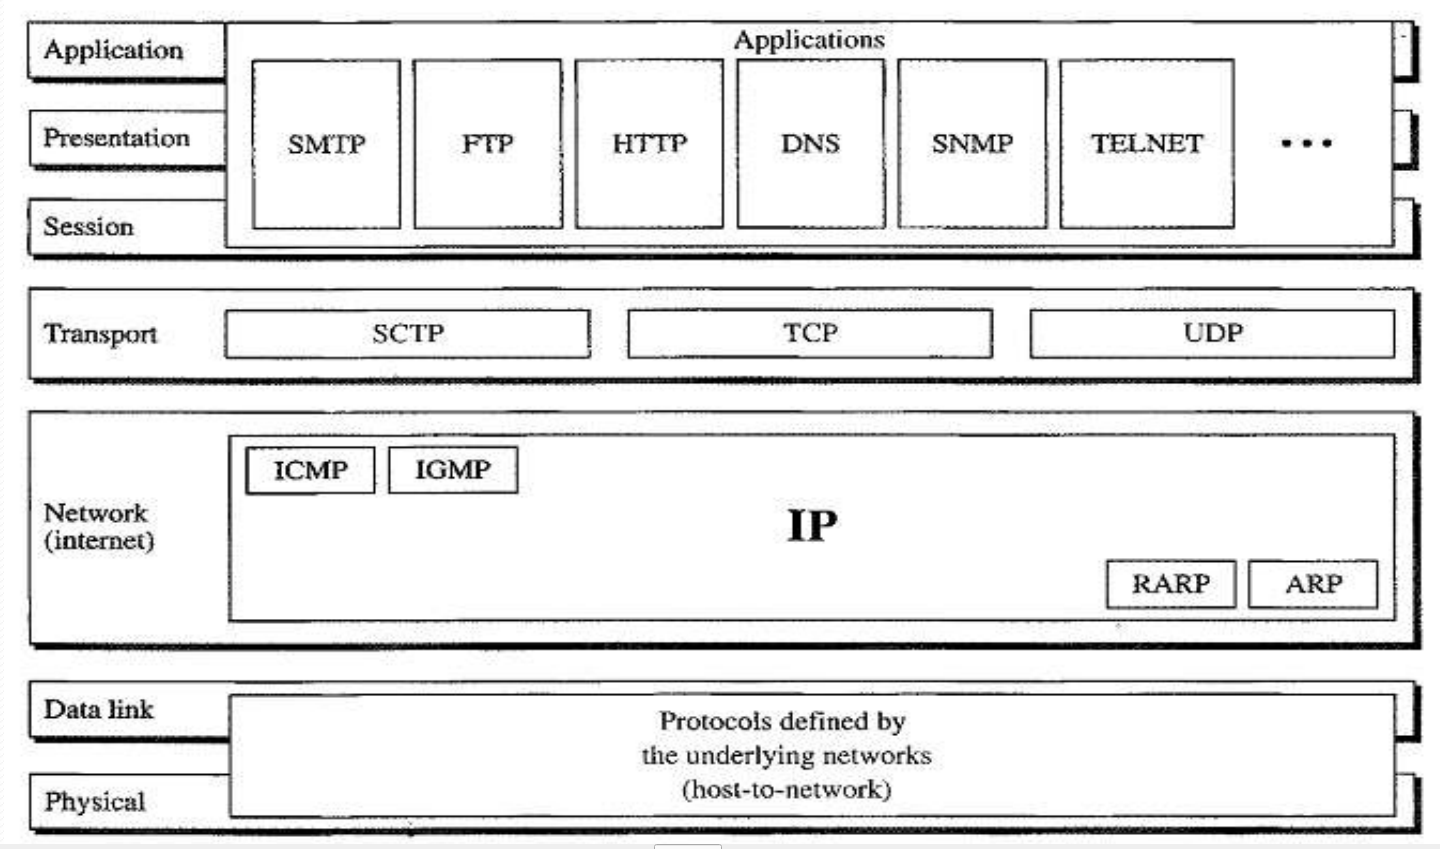
\includegraphics[scale=0.3]{images/4-12.png} 
     	%\vspace*{-0.5em}
		%\caption{Floating gate transistor cell}
	\end{figure}	
	\end{center}
		
	\end{frame}

	\subsection{TCP/IP layers}	
	
	\begin{frame}

	Layer 1: the host to network layer:
	\vspace*{1em}

	\begin{itemize}
	\item{It is the bottom layer of TCP/IP model also known as Network interface layer.}
	\item{The purpose of this layer is to connect the host and the network.}
	\end{itemize}

	\end{frame}

	\begin{frame}
	
	Layer 2: the internet layer
	\vspace*{1em}	
	
	\begin{itemize}
		\item{Internet layer is similar to network layer of OSI model in functionality.}
		\item{This layer is responsible for delivering IP packets to their destinations.}
		\item{An important protocol of this layer is IP (Internet Protocol)}
	\end{itemize}	
			
	\end{frame}

	\begin{frame}
	
	The internet protocol (IP)
	\vspace*{1em}	
	
	\begin{itemize}
		\item{It is an unreliable and connection-less protocol}
		\item{IP transports data in packets called datagrams.}
		\item{IP does no keep track of the routes.}
	\end{itemize}
	
	\end{frame}
		
	\begin{frame}
	
	IP Datagram:
	\vspace*{1em}	
	
	\begin{center}	
	\begin{figure}
		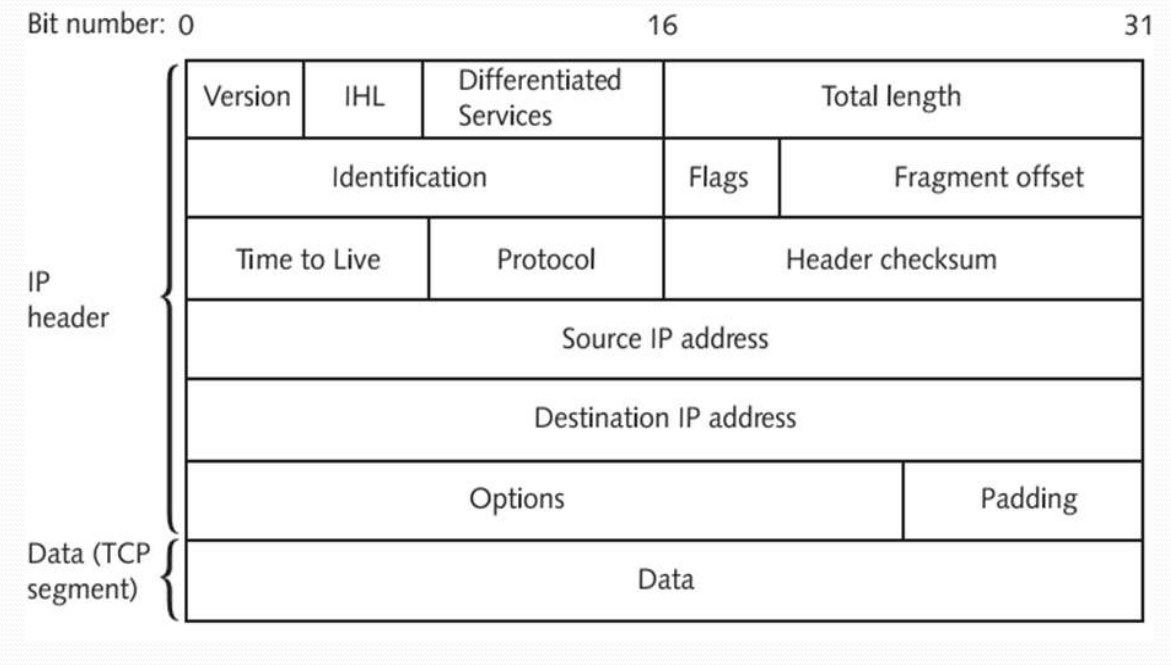
\includegraphics[scale=0.3]{images/4-13.png} 
     	%\vspace*{-0.5em}
		%\caption{Floating gate transistor cell}
	\end{figure}	
	\end{center}	
		
	
	\end{frame}
	
	\begin{frame}
	
	The layer 3: the transport layer
	\vspace*{1em}	
	
	\begin{itemize}
	\item{Transport layer is similar to transport layer of OSI model}
	\item{Transport layer of TCP/IP model also provides connection oriented and connection-less services.
		\begin{itemize}
			\item{Connection Oriented - TCP (Transmission Control Protocol)}
			\item{Connection-less UDP (User Datagram Protocol)}
		\end{itemize}			
	
	}
		
	\end{itemize}	 	
	
	\end{frame}
	
	\begin{frame}

	TCP:
	\vspace*{1em}	
	
	\begin{itemize}
	\item{Transport layer used TCP for reliable connection oriented service}
	\item{The various function of TCP are:
	\begin{itemize}
	\item{Error control}
	\item{Flow control}
	\item{Sequencing}
	\end{itemize}
	
	}
	
	\end{itemize}		
	
	
	\end{frame}
	
	\begin{frame}
	UDP:
	\vspace*{1em}
	
	\begin{itemize}
	\item{Transport layer uses this protocol for unreliable connection-less service.}
	\item{No assurance that all packets reached destination.}
	\item{No sequencing \& No error checking.}
	\item{Useful in real time data transfer and quick transfer of large data (ex: video streaming, etc.)}
	\item{It follows the following principle: delivery is more important than accurate delivery!}
	\end{itemize}
	\end{frame}
	
	\begin{frame}
	
	Application layer:
	\vspace*{1em}	
	
	\begin{itemize}
	\item{This layer is the combination of Application, Presentation and Session layer of the OS	I model.}
	\item{This layer provides various services to different user applications.}
	\end{itemize}		
	
	\end{frame}
	
	\begin{frame}
	
	More about the application layer:
	\vspace*{1em}	
	
	\begin{itemize}
	\item{Application layer includes several high-level protocols that are used for wide variety of application like: 
		\begin{itemize}
			\item{TELNET (Terminal Network): used for remote login.}
			\item{SSH (Secured Shell): used for secured remote login.}
			\item{FTP (File Transfer Protocol): For transfer of file from one system to another.}
			\item{HTTP (Hyper Text Transfer Protocol): For fetching web pages on world wide web.}	
			\item{League Of Legend: For playing with people worldwide.}
			\item{...}	
		\end{itemize}			
	
	}
	\end{itemize}		
	
	
	\end{frame}

	\subsection{Similarities between OSI \& TCP/IP}
	
	\begin{frame}

	Similarities between OSI \& TCP:IP models:
	\vspace{1em}

	\begin{itemize}
		\item{Both are based on the concept of a stack of independent protocols.}
		\item{Functionality of layers are roughly similar.}
		\item{Up to transport: network oriented.}
		\item{Above: user oriented.}
	\end{itemize}
	

	
	\end{frame}

	\subsection{Differences between OSI \& TCP/IP}

	\begin{frame}
	
	Differences between OSI \& TCP/IP models:
	\vspace*{1em}	
	
	\begin{itemize}
	\item{OSI model has seven layers
	\begin{itemize}
	\item{TCP/IP has four layers}
\end{itemize}		
	
	}
	\item{OSI model provides clear distinction between services, interfaces and protocols.
	\begin{itemize}
	\item{TCP/IP doesn't provide clear distinction between services, interface and protocols.}
\end{itemize}		
	
	}
	\item{In OSI model transport layer is connection oriented
	\begin{itemize}
	\item{In TCP/IP transport layer is both connection oriented and connection-less (you can select)}
\end{itemize}		
	
	}
	\end{itemize}

	
	\end{frame}

	\begin{frame}
	
	More differences:
	\vspace*{1em}	
	
	\begin{itemize}
	\item{In OSI the Data Link layer and the Physical layer are separate layers.
		\begin{itemize}
		\item{In TCP/IP the Data Link layer and Physical layer are combined into one: host-to-network layer.}		
		\end{itemize}			
	}
	\item{Protocols do not fit well into the OSI model
	\begin{itemize}
		\item{Protocols fit well with TCP/IP model}
	\end{itemize}}
	\item{Minimum size of OSI header is 5 bytes \begin{itemize}
		\item{In TCP/IP minimum size of the header is 20 bytes.}	
\end{itemize}	 }
\end{itemize}		
	
	\end{frame}



\end{document}